\section{Systematics}
\label{sec:systematics}

The analysis includes both the statistical fit to MD distribution to search the EW-$ZZjj$ process,
as well as the cross section measurement of inclusive EW and QCD $ZZjj$ process in fiducial volume.
Therefore, theoretical and experimental uncertainties may affect the predictions background yields and shapes, 
correction factors from detector-level to particle-level measurement, as well as the $ZZjj$ MD shapes and so on.
Moreover, the statistical uncertainties of simulated samples are also taken into account.
Due to the extremely low cross section of \llll channel, the analysis is still data statistic dominant.
This section describes the measurement of both theoretical and experimental systematics for $ZZjj$ productions.
The systematics for fake backgrounds have been elaborated in section~\ref{sec:fake_syst}.

\subsection{Theoretical systematics}

The theoretical systematics on EW- and QCD-$ZZjj$ processes include the uncertainties from PDF, QCD scale, $\alpha_{S}$ and parton showering variations as summarized in table~\ref{tab:syst_theo_uncer}.
The PDF uncertainty is estimated from the envelop of NNPDF internal variations and the difference between nominal and alternative PDF sets, following the PDF4LHC as introduced in section~\ref{hadroniccollision}.
The QCD scale uncertainty is estimated by varying the nominal renormalization scale ($\mu_{R}$) and factorisation scale ($\mu_{F}$) by a factor of 0.5 or 2.0.
There are seven different configurations being considered, where the maximum of variations is chosen as final uncertainty.
The parton showering uncertainty is estimated by comparing events with different parton showering setting between the nominal \textsc{Pythia8} and the alternative \textsc{Herwig7}\cite{Bellm:2015jjp, Bahr:2008pv} algorithm.
The $\alpha_{S}$ uncertainty is estimated by varying the value of $\alpha_{S}$ within \pm 0.001.
Due to the lack of simulation sample for alternative parton showering on QCD-$ZZjj$ process, 
the value of parton showering component is taken from the measurement of EW process.
\begin{table}[!htb]
\small
\begin{center}
\begin{tabular}{p{5cm}p{5cm}p{5cm}} 
\hline\hline
Process     & EW-$ZZjj$   & QCD-$ZZjj$ \\
\hline
PDFs        & NNPDF30lo (nominal), CT14lo & NNPDF30nnlo (nominal), MMHT2014nnlo68cl, CT14nnlo \\
\hline
$\alpha_{S}$ & 0.118 & 0.117, 0.118 (nominal), 0.119 \\
\hline
QCD scale ([$\mu_{R}$, $\mu_{F}$]) & [0.5,0.5], [0.5,1], [1,0.5], [1,1], [1,2], [2,1], [2,2] & [0.5,0.5], [0.5,1], [1,0.5], [1,1], [1,2], [2,1], [2,2] \\
\hline 
Parton showering algorithm & \textsc{Pythia8}, \textsc{Herwig7} & - \\
\hline\hline
\end{tabular}
\caption{
Summary of different variations for EW- and QCD-$ZZjj$ theoretical uncertainties measurement.
}
\label{tab:syst_theo_uncer}
\end{center}
\end{table}

Table~\ref{tab:syst_theo_sr} summarizes the uncertainties of each theoretical components in fiducial volume of SR,
while table~\ref{tab:syst_theo_cr} shows the numbers in QCD-enriched CR region.
For QCD process, the uncertainty is QCD scale dominant.
Both of them are taken as inputs for statistical fit.
\begin{table}[!htb]
\small
\begin{center}
\begin{tabular}{lllll} 
\hline\hline
Process     & PDF (\%)  & $\alpha_{S}$ (\%) & QCD scale (\%) & Parton shower (\%) \\
\hline
EW         & +5.9 -5.9 &                   & +6.1 -5.6      & +3.3 -3.3          \\
qqQCD      & +2.0 -1.0 & +2.6 -2.6         & +34.2 -22.8    &                    \\
\hline\hline
\end{tabular}
\caption{
Summary of theoretical uncertainties for the fiducial volume (SR) for both EW and QCD $qq$-initial processes.
}
\label{tab:syst_theo_sr}
\end{center}
\end{table}

\begin{table}[!htb]
\small
\begin{center}
\begin{tabular}{lllll} 
\hline\hline
Process      &  PDF (\%)                    & $\alpha_{S}$ (\%)    & QCD scale (\%)                     & Parton shower (\%)  \\
\hline
EW \llll     &  +6.1 -6.1                   &                      & +0.8 -1.1                          & +10.1 -10.1           \\
qqQCD \llll  &  +2.0 -1.0                   & +2.6 -2.6            & +31.5 -22.0                        &                     \\
\hline\hline
\end{tabular}
\caption{
Summary of theoretical uncertainties for the control region for EW and qqQCD processes.
}
\label{tab:syst_theo_cr}
\end{center}
\end{table}
The uncertainties of QCD $gg$-induced process ($gg \rightarrow ZZ$) as the function of MD discriminant is shown in figure~\ref{fig:syst_theo_gg} for both fiducial volume (SR) and QCD CR.
\begin{figure}
  \centering
  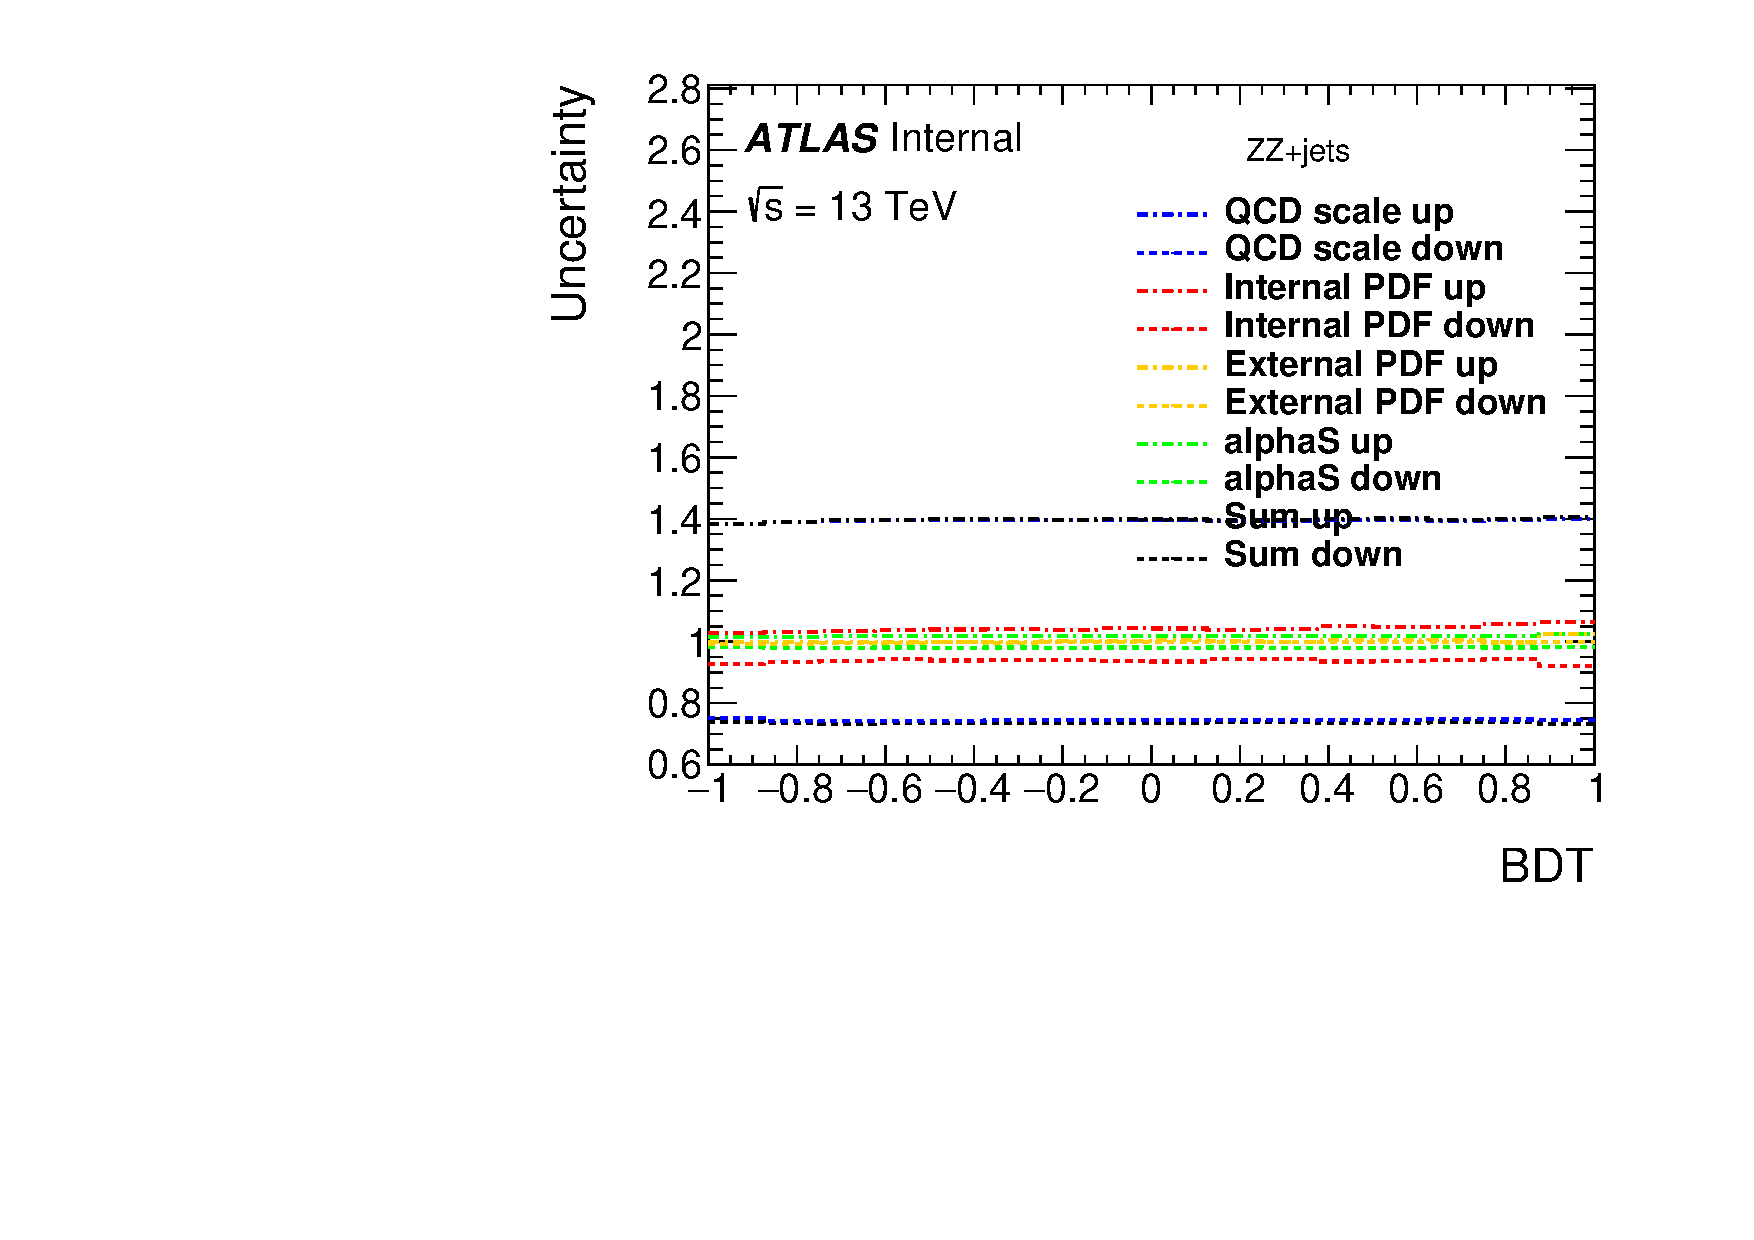
\includegraphics[width=0.42\textwidth]{figures/VBSZZ/syst/BDT_SR_linear.pdf}
  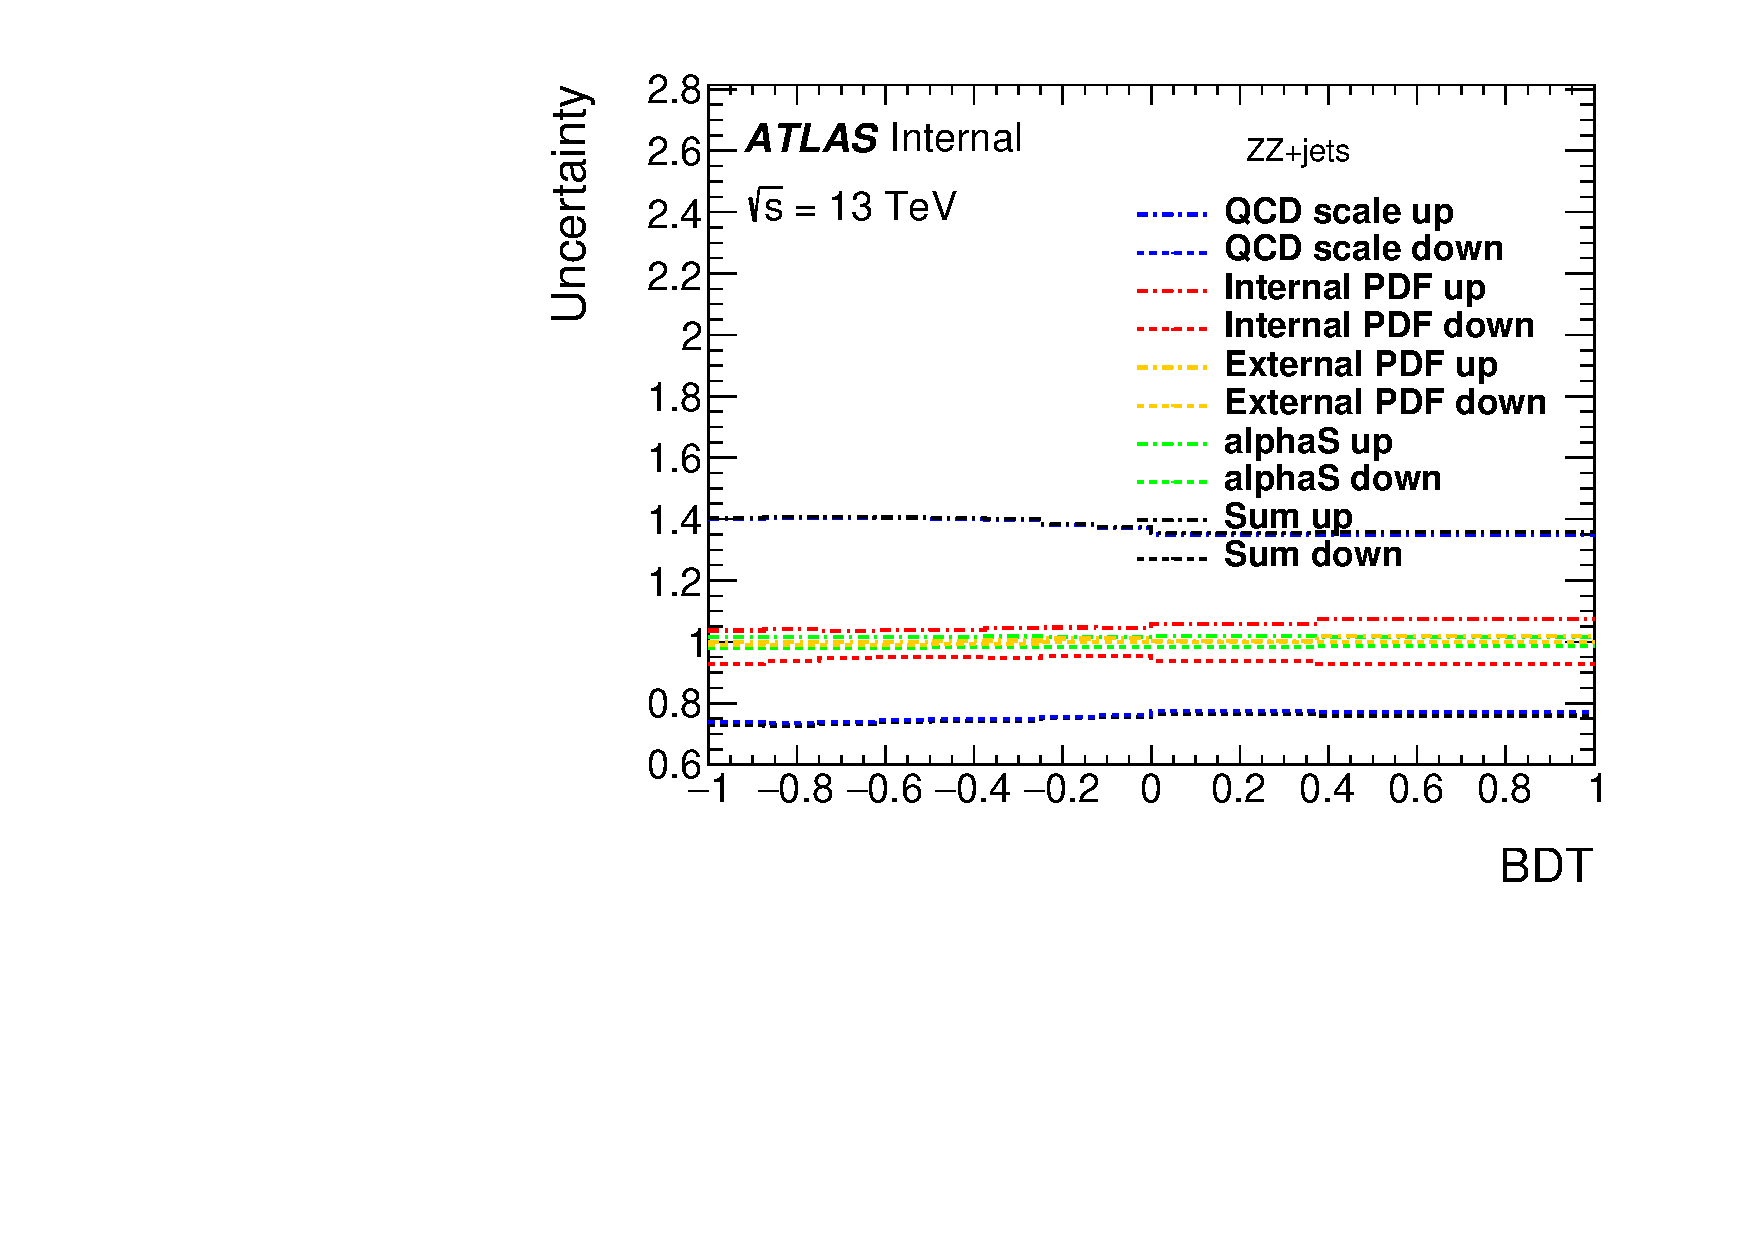
\includegraphics[width=0.42\textwidth]{figures/VBSZZ/syst/BDT_CR_linear.pdf}
  \caption{The theoretical uncertainties for \ggZZ background in particle-level SR (left) and CR (right).}
  \label{fig:syst_theo_gg}
\end{figure}

\subsection{Experimental systematics}
\label{sec:vbszz_exp_uncer}

The diminant experimental uncertainties are from the luminosity uncertainty, the momentum scale and resolution of leptons and jets, as well as the lepton reconstruction and selection efficiency.
Some smaller uncertainties, such as trigger efficiency and pile-up correction, are also considered.
Table~\ref{tab:syst_exp_num} lists the major systematic components from leptons and jets for signal and major background processes in \llll channel.
The total uncertainties for sources from electron, muon and jet respectively, as well as the sum (quadratic sum) of them are also summarized in this table.
\begin{table}[H]
\begin{center}
\small
\begin{tabular}{|c|c|c|c|}
\hline
name&EW-$ZZjj$&QCD $qq$-initial&QCD $gg$\\
\hline
nominal yield&20.61&76.69&13.10\\
\hline
EG\_RESOLUTION\_ALL&$\pm^{0.00\%}_{0.03\%}$&$\pm_{0.04\%}^{0.02\%}$&$\pm^{0.01\%}_{1.41\%}$\\
\hline
EG\_SCALE\_ALL&$\pm^{0.03\%}_{0.05\%}$&-0.04\%&$\pm^{0.01\%}_{0.06\%}$\\
\hline
EL\_EFF\_ID\_TOTAL\_1NPCOR\_PLUS\_UNCOR&$\pm^{2.66\%}_{2.58\%}$&$\pm^{2.60\%}_{2.53\%}$&$\pm^{2.65\%}_{2.57\%}$\\
\hline
EL\_EFF\_Iso\_TOTAL\_1NPCOR\_PLUS\_UNCOR&$\pm$0.70\%&$\pm$0.47\%&$\pm$0.42\%\\
\hline
EL\_EFF\_Reco\_TOTAL\_1NPCOR\_PLUS\_UNCOR&$\pm$0.55\%&$\pm$0.55\%&$\pm$0.63\%\\
\hline
JET\_EtaIntercalibration\_NonClosure&-0.01\%&-0.03\%&0\%\\
\hline
JET\_GroupedNP\_1&$\pm$1.97\%&$\pm^{11.82\%}_{10.14\%}$&$\pm^{16.21\%}_{12.92\%}$\\
\hline
JET\_GroupedNP\_2&$\pm$0.23\%&$\pm$1.26\%&+5.3\%\\
\hline
JET\_GroupedNP\_3&$\pm$0.55\%&$\pm$2.94\%&$\pm^{3.14\%}_{0.12\%}$\\
\hline
JET\_JER\_SINGLE\_NP&0.11\%&+5.47\%&+6.31\%\\
\hline
JET\_JvtEfficiency&$\pm$0.04\%&$\pm$0.12\%&$\pm$0.15\%\\
\hline
MUON\_EFF\_ISO\_STAT&$\pm$0.09\%&$\pm$0.08\%&$\pm$0.07\%\\
\hline
MUON\_EFF\_ISO\_SYS&$\pm$0.54\%&$\pm$0.55\%&$\pm$0.56\%\\
\hline
MUON\_EFF\_RECO\_STAT&$\pm$0.15\%&$\pm$0.19\%&$\pm$0.15\%\\
\hline
MUON\_EFF\_RECO\_STAT\_LOWPT&$\pm$0.06\%&$\pm$0.02\%&$\pm$0.03\%\\
\hline
MUON\_EFF\_TTVA\_STAT&$\pm$0.06\%&$\pm$0.07\%&$\pm$0.06\%\\
\hline
MUON\_EFF\_TTVA\_SYS&$\pm$0.03\%&$\pm$0.4\%&$\pm$0.03\%\\
\hline
MUON\_ID&$\pm$0.03\%&$\pm$0.02\%&$<$0.001\%\\
\hline
MUON\_MS&-0.05\%&$\pm^{0.04\%}_{0.01\%}$&$<$0.001\%\\
\hline
MUON\_SAGITTA\_RESBIAS&$\pm$0.01\%&$\pm$0.02\%&$<$0.001\%\\
\hline
MUON\_SAGITTA\_RHO&+1.13\%&-0.73\%&$\pm$1.00\%\\
\hline
MUON\_SCALE&$\pm$0.02\%&$\pm^{0.03\%}_{0.02\%}$&$<$0.001\%\\
\hline
PRW\_DATASF&$\pm$0.5\%&$\pm^{0.42\%}_{1.02\%}$&$\pm^{2.17\%}_{1.46\%}$\\
\hline
\hline
Electron Exp&$\pm^{2.8\%}_{2.7\%}$&$\pm^{2.70\%}_{2.62\%}$&$\pm^{2.75\%}_{2.64\%}$\\
\hline
Muon Exp&$\pm$1.3\%&$\pm$1.3\%&$\pm$1.04\%\\
\hline
Jet Exp&$\pm$2.0\%&$\pm^{13.39\%}_{10.64\%}$&$\pm^{18.54\%}_{13.57\%}$\\
\hline
\hline
Total experimental uncertainties &$\pm^{3.7\%}_{4.0\%}$&$\pm^{13.72\%}_{11.11\%}$&$\pm^{18.90\%}_{13.57\%}$\\
\hline
\end{tabular}
\caption{
Experimental uncertainties in \llll channel with the luminosity of 139~\ifb.
The "Electron Exp", "Muon Exp" and "Jet Exp" represent the quadrature of the respective sources from electron, muon, and jets.
}
\label{tab:syst_exp_num}
\end{center}
\end{table}

In addition, the uncertainty of the combined 2015 to 2018 integrated luminosity is 1.7\%~\cite{ATLAS-CONF-2019-021} in ATLAS experiment,
obtained using the LUCID-2 detector~\cite{Avoni_2018} for the primary luminosity measurements.

On top of them, a systematic uncertainty for MD distribution with different pile-up (<$\mu$>) is also considered for QCD-$ZZjj$ background
by comparing the distributions between events with low and high pile-up conditions.
A boundary of <$\mu$> = 33 is used to defined low/high pile-up according to the average <$\mu$> for signal (about 34.5) and QCD background (about 33).
Figure~\ref{fig:syst_exp_pu} shows the MD distribution in SR (left) and QCD CR (right) in two different PU conditions, 
the difference as function of MD is then taken into account as additional shape uncertainty for statistical fit.
\begin{figure}[H]
  \centering
  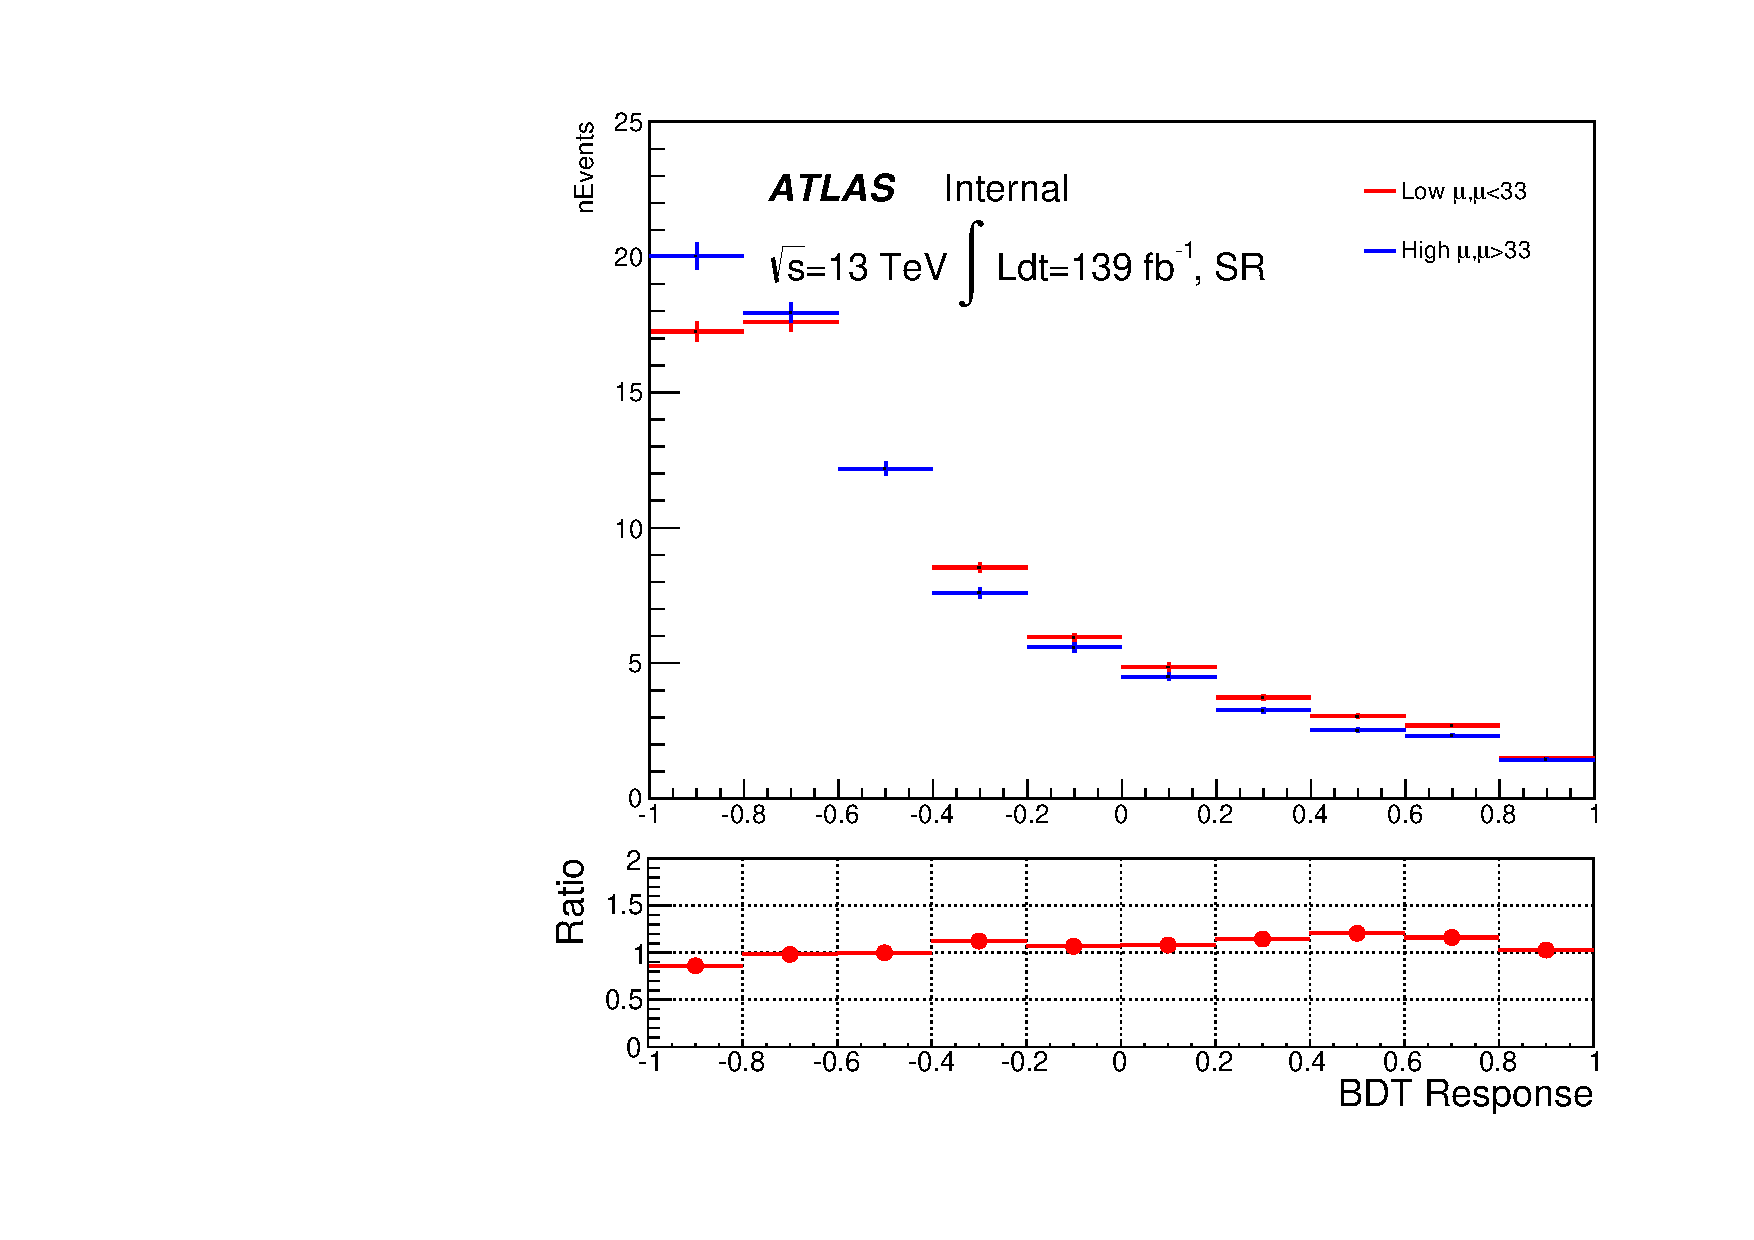
\includegraphics[width=0.42\textwidth]{figures/VBSZZ/syst/pu_uncer_BDT_SR.pdf}
  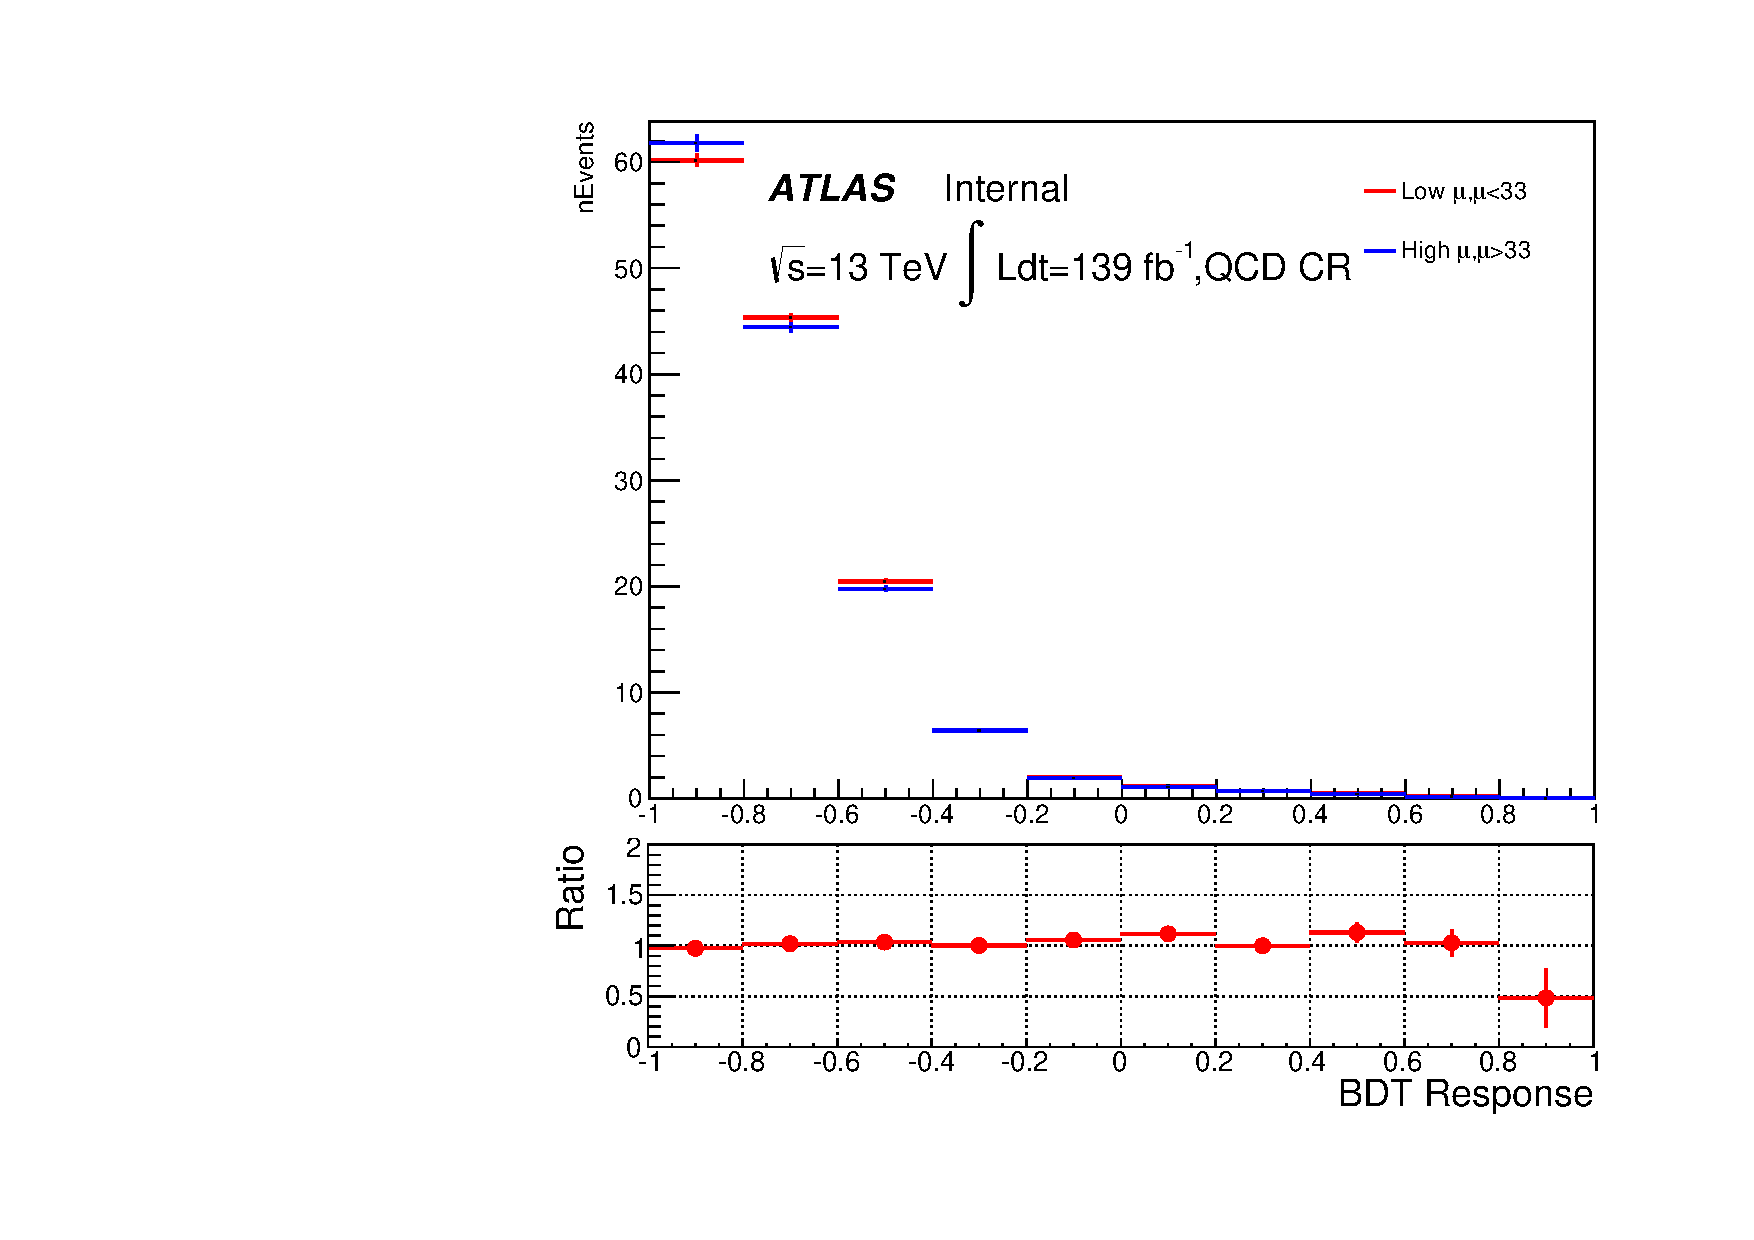
\includegraphics[width=0.42\textwidth]{figures/VBSZZ/syst/pu_uncer_BDT_CR.pdf}
  \caption{MD distribution for QCD-$ZZjj$ process in low and high pile-up events for SR (left) and CR (right).}
  \label{fig:syst_exp_pu}
\end{figure}

Moreover, a conservative uncertainty is signed to QCD-$ZZjj$ process by comparing the sample modelled by \textsc{Sherpa} generator (nominal) with \MGMCatNLO.
The MD shape difference for both SR (left) and QCD CR (right) are shown in figure~\ref{fig:sys_exp_shmg}.
The modelling uncertainty is then calculated from the envelop between nominal and alternative samples as function of MD as one additional shape uncertainty.
\begin{figure}
  \centering
  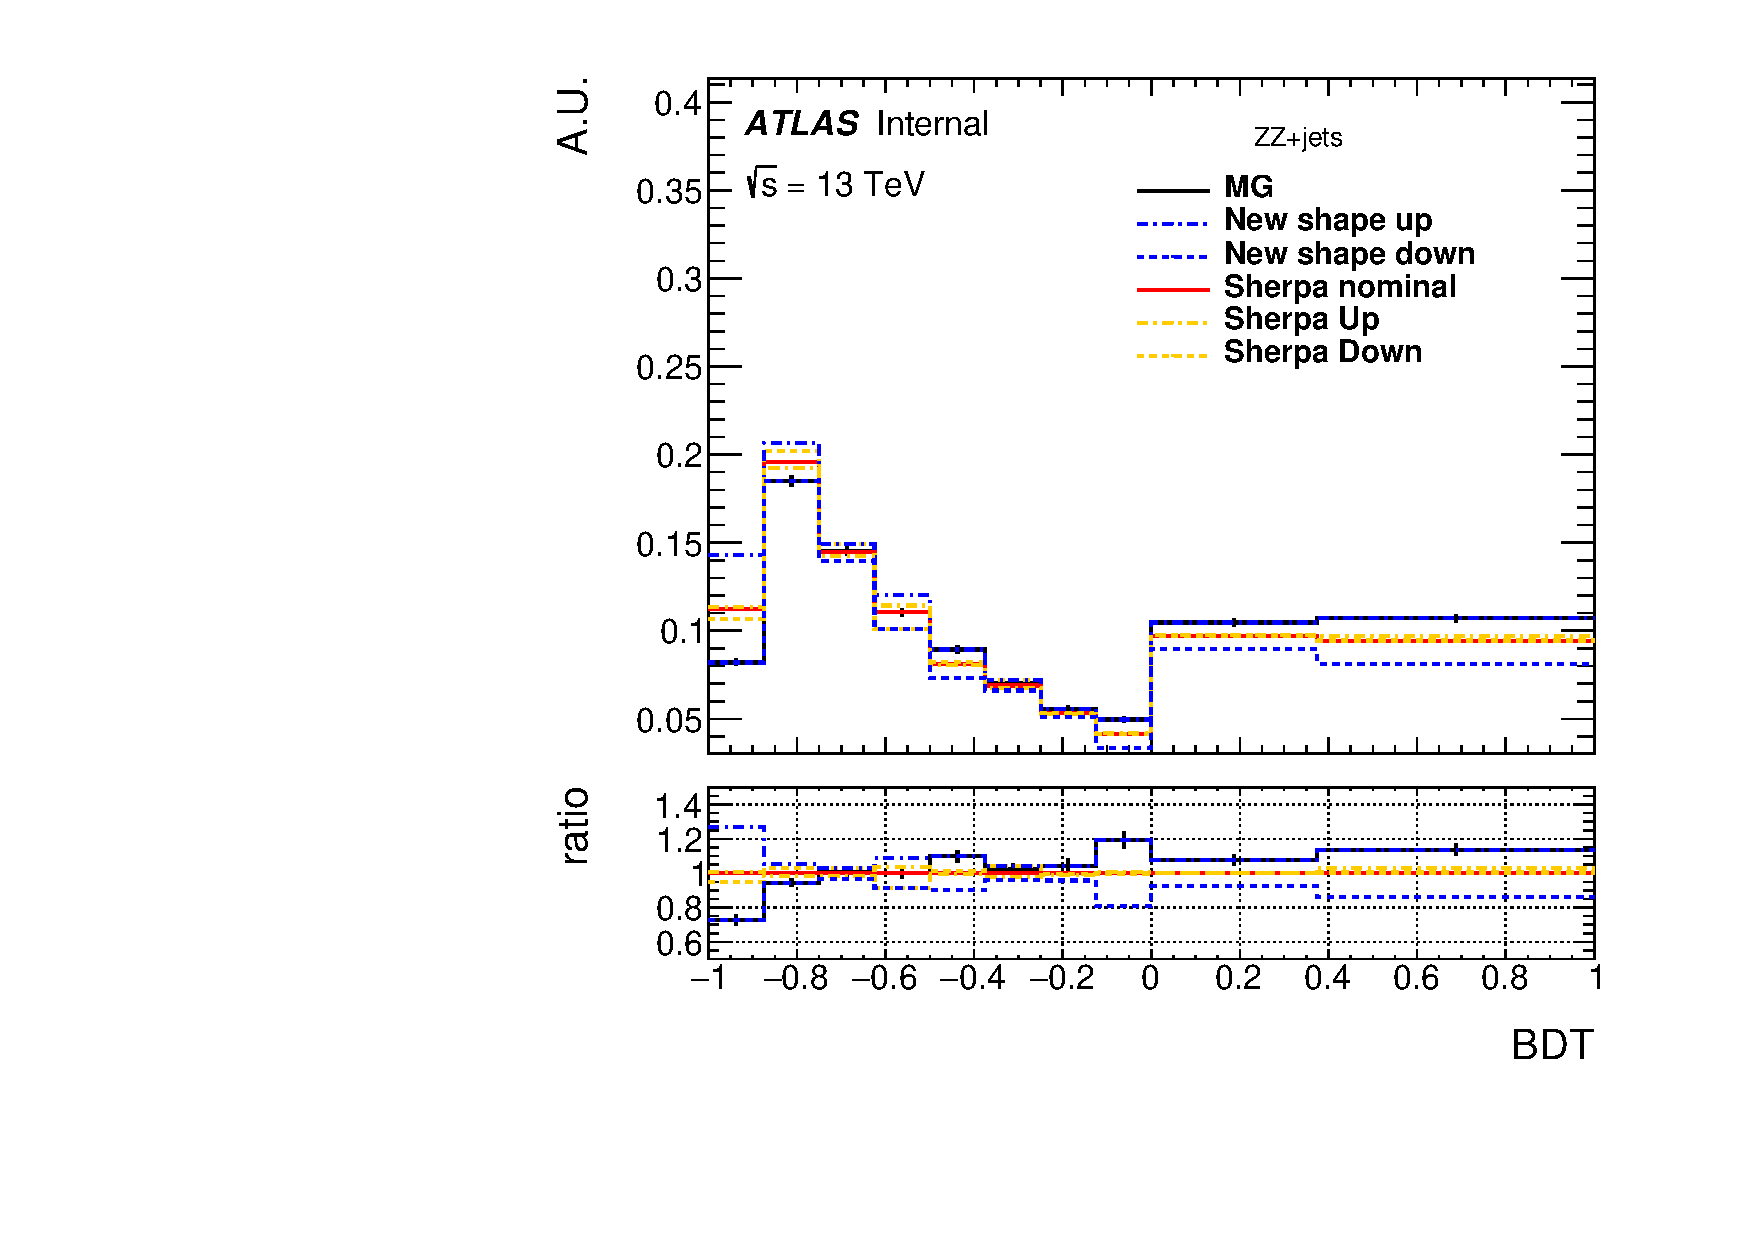
\includegraphics[width=0.42\textwidth]{figures/VBSZZ/syst/BDT_shape_nor_linear_SR.pdf}
  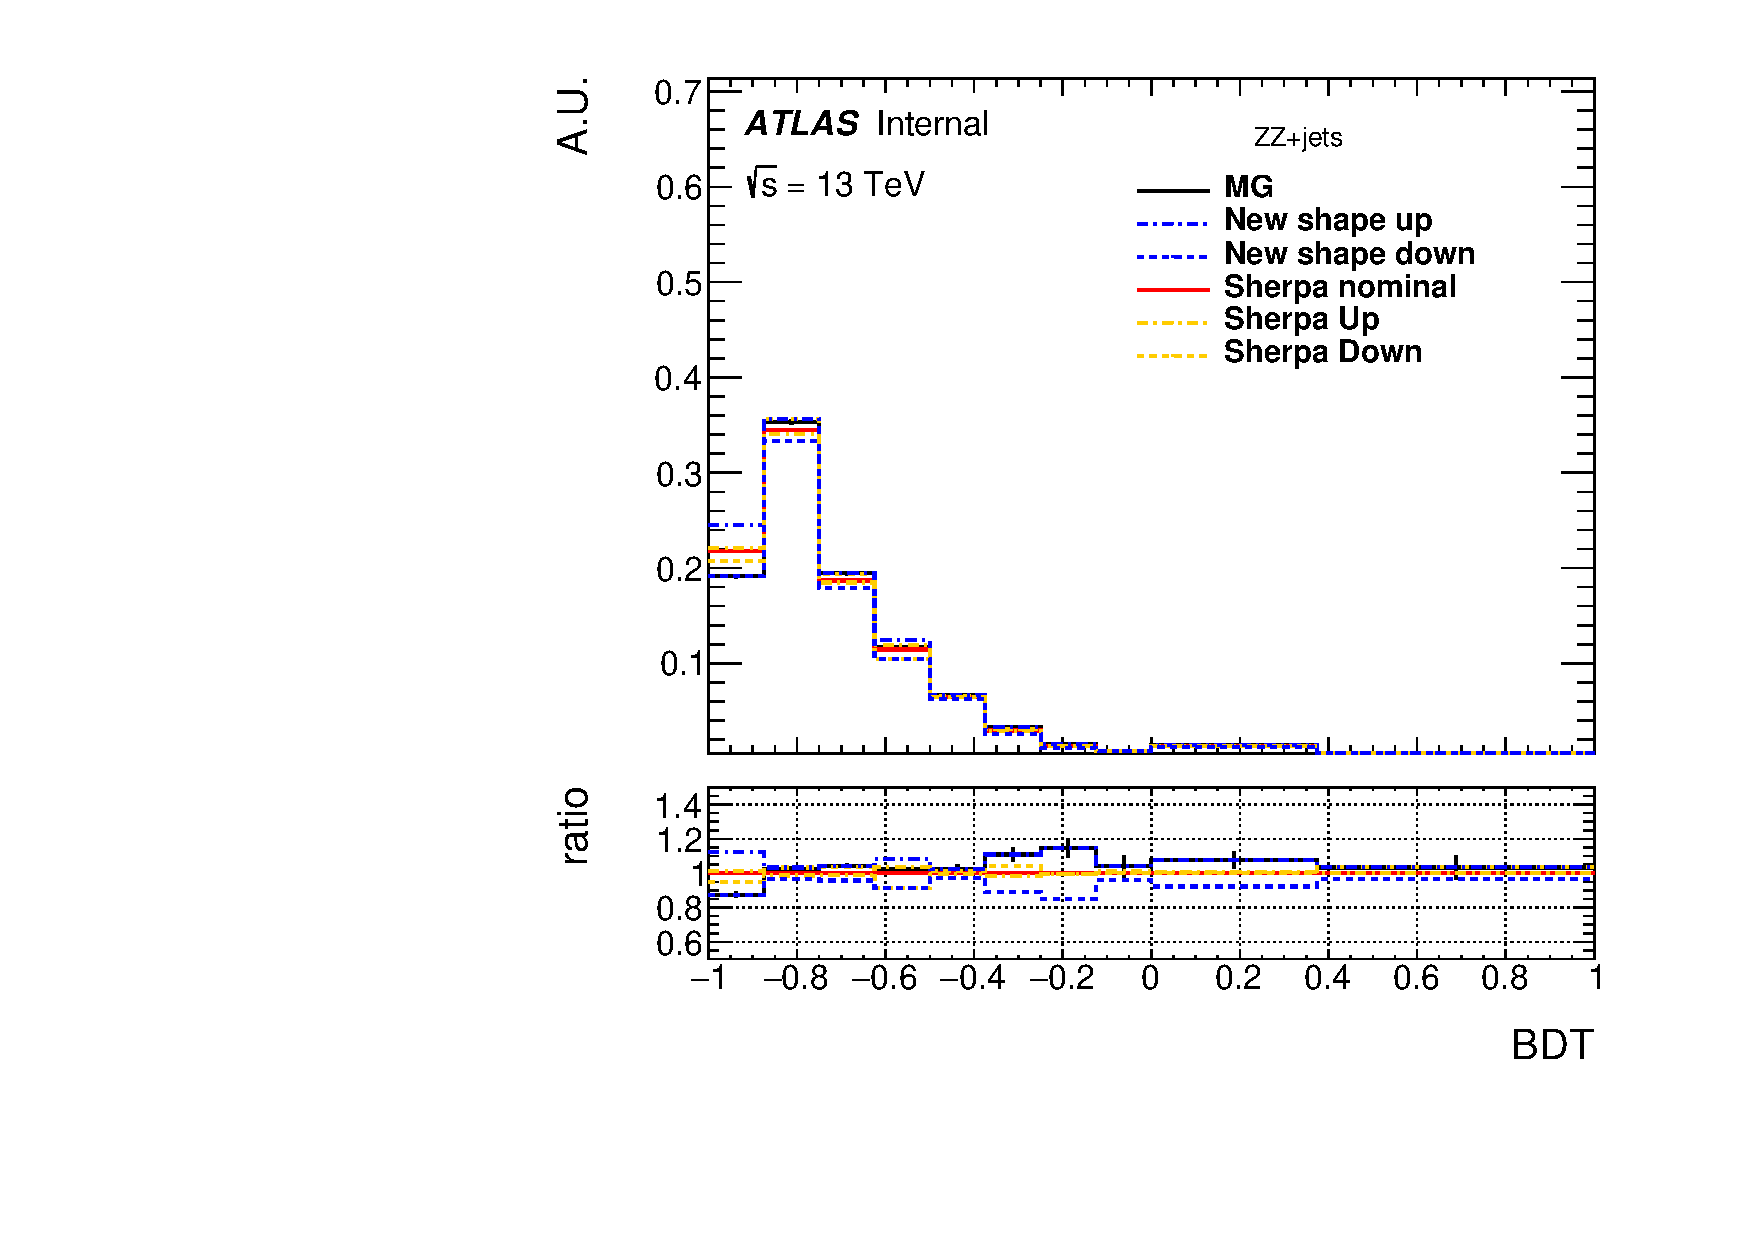
\includegraphics[width=0.42\textwidth]{figures/VBSZZ/syst/BDT_shape_nor_linear_CR.pdf}
  \caption{MD shape difference for QCD \qqZZ background between different \textsc{Sherpa} theoretical uncertainties and sample from \MGMCatNLO on SR (left) and CR (right).}
  \label{fig:sys_exp_shmg}
\end{figure}

